\section{Method}\label{sec:cnn-treelstm}
For composing fixed size presentation vectors of a sentence given a set of variable-length feature maps, one intuitive solution would be to apply Recurrent Neural Networks which have been done by Wang et al.~\cite{cnn-rnn}.
Another solution would be to utilize Recursive Neural Networks.

Different from the leaf module of Constituency Tree-LSTM, CNNs'~\cite{KimCNN,DCNN,2-layer-cnn} first convolution layer have hundreds of filters, each produces a feature map of the sentence by sliding through it with window sizes 3 to 5 words.
Filters with large context window might help CNNs to mitigate the problem of words ambiguity and to capture phrase-level feature.
We think this is the reason why CNNs can outperform TreeLSTMs~\cite{KimCNN}, even when it have no respect for the positions of features. 

We combined Convolution Neural Networks with Constituency Tree-LSTM.
We hypothesized that the convolution layer will help Constituency Tree-LSTM to mitigate the problem of lacking local context and words ambiguity at leaf nodes.
Additionally, using Constituency Tree-LSTM to combine the feature maps produced by the convolution layer might be a better choice compared to using max pooling layers.
\subsection{Model}
Our model has three modules: word embeddings, convolution layer and Constituency Tree-LSTM.
\begin{figure} [H]
	\centering
	\usetikzlibrary{matrix}
\usetikzlibrary{patterns}
\tikzset{
	sq1/.style={rectangle, minimum width=0.5cm, minimum height=0.5cm, text centered, draw=black},
	sq1m/.style={rectangle, minimum width=0.7cm, minimum height=0.3cm, text centered, draw=black},
	sq1p/.style={rectangle, minimum width=0.5cm, minimum height=0.5cm, text centered, draw=black, pattern=north west lines},
	circ/.style={circle, minimum width=0.3cm, minimum height=0.3cm, text centered, draw=black},
	arrow/.style={thick,->},
	sqvec/.style={matrix,matrix of nodes,nodes in empty cells},
}
\tikzstyle{cir} = [circle, minimum width=0.7cm, minimum height=0.7cm, text centered, draw=black ]

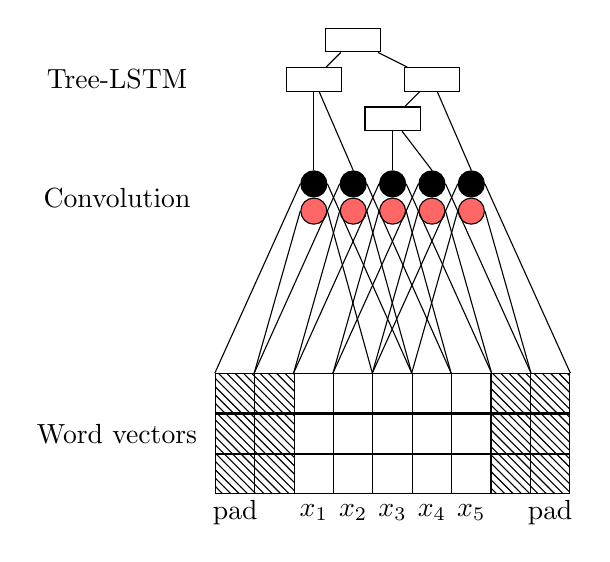
\begin{tikzpicture}
\node [sqvec,nodes={circ},      
every even row/.style = { nodes={fill=red!60}},
every odd row/.style = { nodes={fill=black!100}}] (c1) at (1.5,8.5) {
	\\
	\\ 
};  

\node [sqvec,nodes={circ},      
every even row/.style = { nodes={fill=red!60}},
every odd row/.style = { nodes={fill=black!100}}] (c2) at (2,8.5) {
	\\
	\\ 
};  

\node [sqvec,nodes={circ},      
every even row/.style = { nodes={fill=red!60}},
every odd row/.style = { nodes={fill=black!100}}] (c3) at (2.5,8.5) {
	\\
	\\ 
};  

\node [sqvec,nodes={circ},      
every even row/.style = { nodes={fill=red!60}},
every odd row/.style = { nodes={fill=black!100}}] (c4) at (3,8.5) {
	\\
	\\ 
};  

\node [sqvec,nodes={circ},      
every even row/.style = { nodes={fill=red!60}},
every odd row/.style = { nodes={fill=black!100}}] (c5) at (3.5,8.5) {
	\\
	\\ 
};  


\node [sqvec,column sep=-\pgflinewidth,nodes={sq1}] (v) at (2.5,5.5) {
	&&&&\\
	&&&&\\
	&&&&\\
};   

\node [sqvec,column sep=-\pgflinewidth,nodes={sq1p}] (v1) at (1,5.5) {
	\\
	\\
	\\
};   
\node [sqvec,column sep=-\pgflinewidth,nodes={sq1p}] (v2) at (0.5,5.5) {
	\\
	\\
	\\
};   
\node [sqvec,column sep=-\pgflinewidth,nodes={sq1p}] (v3) at (4,5.5) {
	\\
	\\
	\\
};   
\node [sqvec,column sep=-\pgflinewidth,nodes={sq1p}] (v4) at (4.5,5.5) {
	\\
	\\
	\\
};   

\draw (v1-1-1.north west) -- (c1-2-1.west); % inner left
\draw (v-1-3.north west) -- (c1-2-1.east); % inner right
\draw (v2-1-1.north west) -- (c1-1-1.west); % outer left
\draw (v-1-4.north west) -- (c1-1-1.east); % outer right

\draw (v-1-1.north west) -- (c2-2-1.west); % inner left
\draw (v-1-4.north west) -- (c2-2-1.east); % inner right
\draw (v1-1-1.north west) -- (c2-1-1.west); % outer left
\draw (v-1-5.north west) -- (c2-1-1.east); % outer right

\draw (v-1-2.north west) -- (c3-2-1.west); % inner left
\draw (v-1-5.north west) -- (c3-2-1.east); % inner right
\draw (v-1-1.north west) -- (c3-1-1.west); % outer left
\draw (v-1-5.north east) -- (c3-1-1.east); % outer right

\draw (v-1-3.north west) -- (c4-2-1.west); % inner left
\draw (v-1-5.north east) -- (c4-2-1.east); % inner right
\draw (v-1-2.north west) -- (c4-1-1.west); % outer left
\draw (v3-1-1.north east) -- (c4-1-1.east); % outer right

\draw (v-1-4.north west) -- (c5-2-1.west); % inner left
\draw (v3-1-1.north east) -- (c5-2-1.east); % inner right
\draw (v-1-3.north west) -- (c5-1-1.west); % outer left
\draw (v4-1-1.north east) -- (c5-1-1.east); % outer right


\node [sq1m] (v8) at (2,10.5) {};
\node [sq1m] (v7) at (1.5,10) {};
\node [sq1m] (v6) at (3,10) {};
\node [sq1m] (v5) at (2.5,9.5) {};
% \draw  (c3) edge (v5);
% \draw  (c4) edge (v5);
\draw  (v5) edge (v6);
% \draw  (c5) edge (v6);
% \draw  (c1) edge (v7);
\draw  (v7) edge (v8);
% \draw  (c2) edge (v7);
\draw  (v6) edge (v8);



\node at (0.5,4.5) {pad};
% \node at (1,4) {pad};
\node at (1.5,4.5) {$x_1$};
\node at (2,4.5) {$x_2$};
\node at (2.5,4.5) {$x_3$};
\node at (3,4.5) {$x_4$};
\node at (3.5,4.5) {$x_5$};
\node at (4.5,4.5) {pad};
% \node at (4.5,4) {pad};

\node at (-1,8.5) {Convolution};
\node at (-1,5.5) {Word vectors};
\node at (-1,10) {Tree-LSTM};

% connect lstm to circle
\draw  (v7) edge (c1-1-1.north);
\draw  (v7) edge (c2-1-1.north);
\draw  (v5) edge (c3-1-1.north);
\draw  (v5) edge (c4-1-1.north);
\draw  (v6) edge (c5-1-1.north);
\end{tikzpicture}
	\caption[qwerty]{CNN-Tree-LSTM}
\end{figure}
\subsubsection{Convolution Layer}
We reuse the definition of convolution layer which is described in Sec.~\ref{conv-layer}.
For working with Constituency Tree-LSTM, after going though the convolution layer, the parse tree structure of sentence \(s\) must be applicable on the output of the convolution layer. 
For this purpose, we constrained all the feature maps produced by the convolution layer to have length equal to that of the sentence \(s\) (which is \(n\) in this case).
Additionally, all filters in \(F\) are restricted to have odd window sizes and being applied on the sentence according to half padding, unit strides policy~\cite{conv-arith}.
These conditions entail \({\forall u \in F,  c^{(u)} \in \mathbb{R}^n}\)~\cite{conv-arith}.

Suppose the size of set of filters \(F\) is \(m\), all the feature maps produced by the set of filters is then concatenated into one matrix \(P \in \mathbb{R}^{m \times n}\), which each of its row is a feature maps.
After that, the column vectors of \(P\) are treated as input vectors for the Constituency Tree-LSTM.
\subsubsection{Constituency Tree-LSTM}
The definition of Constituency Tree-LSTM which is described in Sec.~\ref{treelstm} is reused.
The only difference is that for any word-\(i\)th in the sentence, the vector representation of it is the \(i\)th-column of the matrix \(P\) produced by the convolution layer.
This mean the size of any input vector for the Constituency Tree-LSTM is equal to the number of filters \(m\).
\subsection{Model Enhancement}
We observed that the available amount of document-level labeled sentiment data (e.g. Amazon Reviews dataset~\cite{amazon-reviews} has 83.68 million reviews) is gigantic compared to the amount of sentence or phrase-level sentiment data (e.g. Stanford Sentiment Treebank~\cite{socher2013recursive} has 8544 sentences in its training set, even it is the biggest sentence-level sentiment analysis dataset).
Although, there are some attempts to do transfer learning~\cite{group-instance}~\cite{re-embedding} (i.e. training on large document-level sentiment dataset then fine-tuning and/or test on sentence-level sentiment dataset), their performances are not high when evaluated on Stanford Sentiment Treebank~\cite{group-instance}.

We utilized Glove~\cite{glove} method to do transfer learning.
We hypothesized that by training Glove on review documents, especially movie or book reviews, we can capture more rare words and also the different way people use words (or different word relationships) to express their opinions on movies or books.
This might help our models archiving better generalization when training on small sentence-level sentiment dataset like Stanford Sentiment Treebank~\cite{socher2013recursive}.